\documentclass[a4paper,12pt]{article}
\usepackage{graphicx}
\usepackage[a4paper,margin=1in]{geometry}
\usepackage{titlesec}
\usepackage{hyperref}
\usepackage{amsmath}    % For math environments and symbols
\usepackage{amssymb}    % For \mathbb and other math symbols
\usepackage{amsfonts}   % Additional math fonts
\usepackage[backend=biber,style=numeric,sorting=none]{biblatex}

\addbibresource{references.bib} % Add references.bib with the appropriate entries

% Title format
\titleformat{\section}{\large\bfseries}{\thesection}{1em}{}

% Title settings
\title{
    \includegraphics[scale=0.4]{Cam_logo_bw.png}\\
    \vspace{0.5cm}
    C1 Research Computing - Coursework Assignment
}
\author{Raunaq Rai (rsr45@cam.ac.uk)\\
    Department of Physics, University of Cambridge
}
\date{18 December, 2024}

\begin{document}

\maketitle

\section{Introduction}
This report details the development and implementation of a Python package, \texttt{dual\_autodiff}, designed for automatic differentiation using dual numbers. The package computes derivatives efficiently while supporting mathematical operations such as trigonometric, logarithmic, and exponential functions.

The approach builds on the concept of forward-mode automatic differentiation, which is essential in fields like optimization, computational physics, and machine learning. This technique traces its roots to the foundational work by Wengert~\cite{wengert1964automatic}, who introduced a systematic way to compute derivatives using intermediate variables. More recently, Baydin et al.~\cite{baydin2018automatic} surveyed the use of automatic differentiation in machine learning, emphasizing its importance in training deep neural networks.

To enhance performance, a Cython-optimized version, \texttt{dual\_autodiff\_x}, was also developed. This document covers the structure of the project, the mathematical principles behind dual numbers, and the implementation details of the package.

\section{Setting Up the Development Environment}

Apple Silicon devices primarily use the ARM64 architecture, which can pose challenges when working with scientific computing tools built for x86\_64. To ensure compatibility with these tools, I configured the development environment to run in x86\_64 mode. This step was crucial for enabling seamless execution of packages and tools designed for x86\_64 systems.

To achieve this:
\begin{itemize}
    \item \textbf{Rosetta Installation:} Rosetta, an emulation layer by Apple, was installed to facilitate running x86\_64 binaries on ARM-based devices. This was achieved using:
    \begin{verbatim}
    /usr/sbin/softwareupdate --install-rosetta
    \end{verbatim}
    \item \textbf{Configuring Terminal:} The Terminal application was set to run in Rosetta mode, ensuring compatibility with x86\_64 libraries and tools.
    \item \textbf{Creating an x86\_64 Conda Environment:} A dedicated Conda environment was created with all required dependencies for developing and testing the package.
\end{itemize}

This setup allowed for consistent development and ensured the compatibility of tools and libraries required for this project.

\section{Theoretical Background}

\subsection{Dual Numbers}
Dual numbers can be defined as truncated Taylor series of the form:
\[
x = v + \dot{v}\epsilon,
\]
where \(v, \dot{v} \in \mathbb{R}\), and \(\epsilon\) is a nilpotent number such that \(\epsilon^2 = 0\) and \(\epsilon \neq 0\). Here:
\begin{itemize}
    \item \(v\): Represents the \textit{primal value}.
    \item \(\dot{v}\): Represents the \textit{derivative} or \textit{tangent value}.
\end{itemize}

As explained by Baydin et al.~\cite{baydin2018automatic}, arithmetic operations with dual numbers align naturally with symbolic differentiation principles:
\[
(x_1 + \dot{x}_1\epsilon) + (x_2 + \dot{x}_2\epsilon) = (x_1 + x_2) + (\dot{x}_1 + \dot{x}_2)\epsilon,
\]
\[
(x_1 + \dot{x}_1\epsilon)(x_2 + \dot{x}_2\epsilon) = x_1x_2 + (x_1\dot{x}_2 + \dot{x}_1x_2)\epsilon.
\]

\subsection{Automatic Differentiation}
Automatic differentiation (AD) leverages dual numbers to compute derivatives efficiently. For a function \(f(x)\), substituting \(x = v + \dot{v}\epsilon\) yields:
\[
f(x) = f(v + \dot{v}\epsilon) = f(v) + f'(v)\dot{v}\epsilon.
\]
The derivative \(f'(v)\) is embedded in the coefficient of \(\epsilon\), enabling simultaneous evaluation of function values and derivatives.

This principle extends to composite functions via the chain rule:
\[
f(g(v + \dot{v}\epsilon)) = f(g(v)) + f'(g(v))g'(v)\dot{v}\epsilon.
\]

\section{Implementation of Dual Numbers and Operations}

\subsection{Overview of the \texttt{Dual} Class}
The \texttt{dual.py} file implements the \texttt{Dual} class, the core of the \texttt{dual\_autodiff} package. This class defines dual numbers and supports operations such as addition, subtraction, multiplication, and division.

\subsubsection{Arithmetic Operations}
The \texttt{Dual} class overrides arithmetic operators for seamless integration. For example:
\begin{verbatim}
x = Dual(2, 1)
y = Dual(3, 2)
print(x + y)  # Output: Dual(real=5, dual=3)
\end{verbatim}

\subsubsection{Mathematical Functions}
The \texttt{Dual} class also implements key mathematical functions such as:
\begin{itemize}
    \item Trigonometric functions (\texttt{sin}, \texttt{cos}, \texttt{tan}).
    \item Exponential and logarithmic functions (\texttt{exp}, \texttt{log}).
    \item Hyperbolic functions (\texttt{sinh}, \texttt{cosh}, \texttt{tanh}).
    \item Square root (\texttt{sqrt}).
\end{itemize}
For example:
\begin{verbatim}
x = Dual(2, 1)
result = x.sin()
print(result)  # Output: Dual(real=0.9092..., dual=-0.4161...)
\end{verbatim}

\subsection{Utility Functions}
To enhance usability:
\begin{itemize}
    \item \texttt{functions.py} provides aliases for mathematical functions.
    \item \texttt{base.py} includes helper functions like:
    \begin{itemize}
        \item \texttt{is\_dual\_instance(value)}: Checks if a value is a \texttt{Dual} instance.
        \item \texttt{ensure\_dual(value)}: Wraps non-\texttt{Dual} values into a \texttt{Dual} object.
    \end{itemize}
\end{itemize}

\section{Project Structure and Packaging}

\subsection{Repository Organization}
The repository adheres to established best practices for Python projects to ensure clarity, maintainability, and modularity. Below is an overview of its structure:

\subsubsection{Top-Level Directory}
The top-level directory organizes the project as follows:
\begin{itemize}
    \item \textbf{\texttt{dual\_autodiff/}}: Core implementation, including modules like \texttt{dual.py}, \texttt{functions.py}, and \texttt{base.py}.
    \item \textbf{\texttt{tests/}}: Unit tests for core modules.
    \item \textbf{\texttt{docs/}}: Documentation files, including Sphinx configurations.
    \item \textbf{\texttt{report/}}: LaTeX report and related files.
    \item \textbf{\texttt{dist/}}: Package distribution files (wheel and source archives).
    \item \textbf{\texttt{build/}}: Temporary build files.
    \item \textbf{\texttt{pyproject.toml}}: Modern Python project configuration.
    \item \textbf{\texttt{requirements.txt}}: Python dependencies.
    \item \textbf{\texttt{environment.yaml}}: Conda environment definition.
    \item \textbf{\texttt{README.md}}: Project overview and instructions.
\end{itemize}


\subsection{Building and Installing the Package}
The \texttt{pyproject.toml} file is used to manage the configuration and metadata of the project. It follows the modern Python packaging standards and includes the following sections:
\begin{itemize}
    \item \texttt{[build-system]}: Specifies the tools required for building the package, such as \texttt{setuptools} and \texttt{wheel}.
    \item \texttt{[project]}: Contains metadata, including the project name, version, author, and dependencies.
    \item \texttt{[tool.setuptools\_scm]}: Enables dynamic versioning based on the state of the repository.
\end{itemize}

To build and install the package, the following steps were performed:
\begin{enumerate}
    \item Install build tools: \texttt{pip install build}.
    \item Build distributions: \texttt{python -m build}.
    \item Install in editable mode: \texttt{pip install -e .}.
\end{enumerate}

This approach ensures the package is properly configured, packaged, and ready for distribution or further development.

\section{Implementation of \texttt{dual.py}}

\begin{itemize}
    \item \textbf{Arithmetic Operations:} Operators (\texttt{+}, \texttt{-}, \texttt{*}, \texttt{/}) for mathematical operations. For example:
    \begin{verbatim}
    x = Dual(2, 1); y = Dual(3, 2)
    z = x + y  # Dual(real=5, dual=3)
    \end{verbatim}
    \item \textbf{Mathematical Functions:} Implements \texttt{sin}, \texttt{cos}, \texttt{log}, \texttt{exp}, \texttt{sqrt}, etc., extended to dual numbers. For instance:
    \begin{verbatim}
    x = Dual(2, 1)
    result = x.sin()  # Dual(real=0.9092..., dual=-0.4161...)
    \end{verbatim}
    \item \textbf{Power and Root:} Supports scalar powers and square root computations:
    \begin{verbatim}
    x = Dual(4, 1)
    result = x.sqrt()  # Dual(real=2.0, dual=0.25)
    \end{verbatim}
    \item \textbf{Error Handling:} Ensures mathematical operations like \texttt{log} and \texttt{sqrt} are only applied within valid domains.
\end{itemize}

Example:
\[
f(x) = \log(x) + x^2 \implies f'(x) = \frac{1}{x} + 2x
\]
can be evaluated directly using:
\begin{verbatim}
x = Dual(2, 1)
f_x = x.log() + x**2  # Dual(real=4.0, dual=2.5)
\end{verbatim}

\section{Publishing to PyPI}

To make the \texttt{dual\_autodiff} package publicly available, it was uploaded to the Python Package Index (PyPI). The following steps outline the publishing process and installation instructions.

\subsection{Publishing to PyPI}

To publish the \texttt{dual\_autodiff} package on PyPI, the following steps were followed:

\begin{enumerate}
    \item \textbf{Create Distributions:}
    Build source and wheel distributions as done previously:

    \item \textbf{Upload to PyPI:}
    Use \texttt{twine} to securely upload distributions.
    
    Authentication with PyPI credentials was required.

    \item \textbf{Verify Upload:}
    \url{https://pypi.org/project/rsr45-dual-autodiff/}
\end{enumerate}

\subsection{Installing the Package}
Install the package via \texttt{pip}:
\begin{verbatim}
pip install rsr45-dual-autodiff
\end{verbatim}

\subsection{Testing the Installation}
Verify functionality:
\begin{verbatim}
import dual_autodiff as df
x = df.Dual(2, 1)
print(x.sin())
\end{verbatim}



\section{Differentiating a Function}

\subsection{Function Definition}
The target function for differentiation is:
\[
f(x) = \log(\sin(x)) + x^2 \cos(x)
\]
The derivative of this function, computed analytically, is:
\[
f'(x) = -x^2 \sin(x) + \frac{\cos(x)}{\sin(x)} + 2x \cos(x)
\]

\subsection{Using Dual Numbers for Differentiation}
To compute \(f'(x)\) at \(x = 1.5\) using dual numbers:
\begin{itemize}
    \item Represent \(x\) as a dual number: \(x = 1.5 + 1\epsilon\), where the real part is \(1.5\) and the dual part represents the derivative.
    \item Substitute \(x\) into \(f(x)\) and use the dual number arithmetic to compute \(f'(x)\) from the dual part of the result.
\end{itemize}

\subsection{Results}

\subsubsection{Using Dual Numbers}
The function \(f(x)\) and its derivative \(f'(x)\) were computed at \(x = 1.5\) using dual numbers. The results are as follows:
\[
f(1.5) = 0.15665054756073515, \quad f'(1.5) = -1.9612372705533612
\]

\subsubsection{Using Manual Computation}
The analytical expression for \(f(x)\) and \(f'(x)\) was used to compute the same values at \(x = 1.5\). The results are:
\[
f(1.5) = 0.15665054756073515, \quad f'(1.5) = -1.9612372705533614
\]

\subsubsection{Comparison}
The results obtained using dual numbers closely match the manually computed values, confirming the correctness of the dual number implementation. The slight discrepancy in the derivative (\(2 \times 10^{-13}\)) is attributed to floating-point precision errors inherent in numerical computations.

\subsection{Comparison with Numerical Differentiation}

\begin{itemize}
    \item \textbf{Numerical Differentiation:} The central difference formula was used:
    \[
    f'(x) \approx \frac{f(x + h) - f(x - h)}{2h}.
    \]
    This was evaluated for step sizes decreasing logarithmically from \(h = 10^{-0.5}\) to \(h = 10^{-3}\).
\end{itemize}

Figure~\ref{fig:convergence_derivative} illustrates the behavior of the numerical derivative as the step size decreases. The red dashed line represents the true derivative obtained using dual numbers, which serves as the reference value.

\begin{figure}[h!]
    \centering
    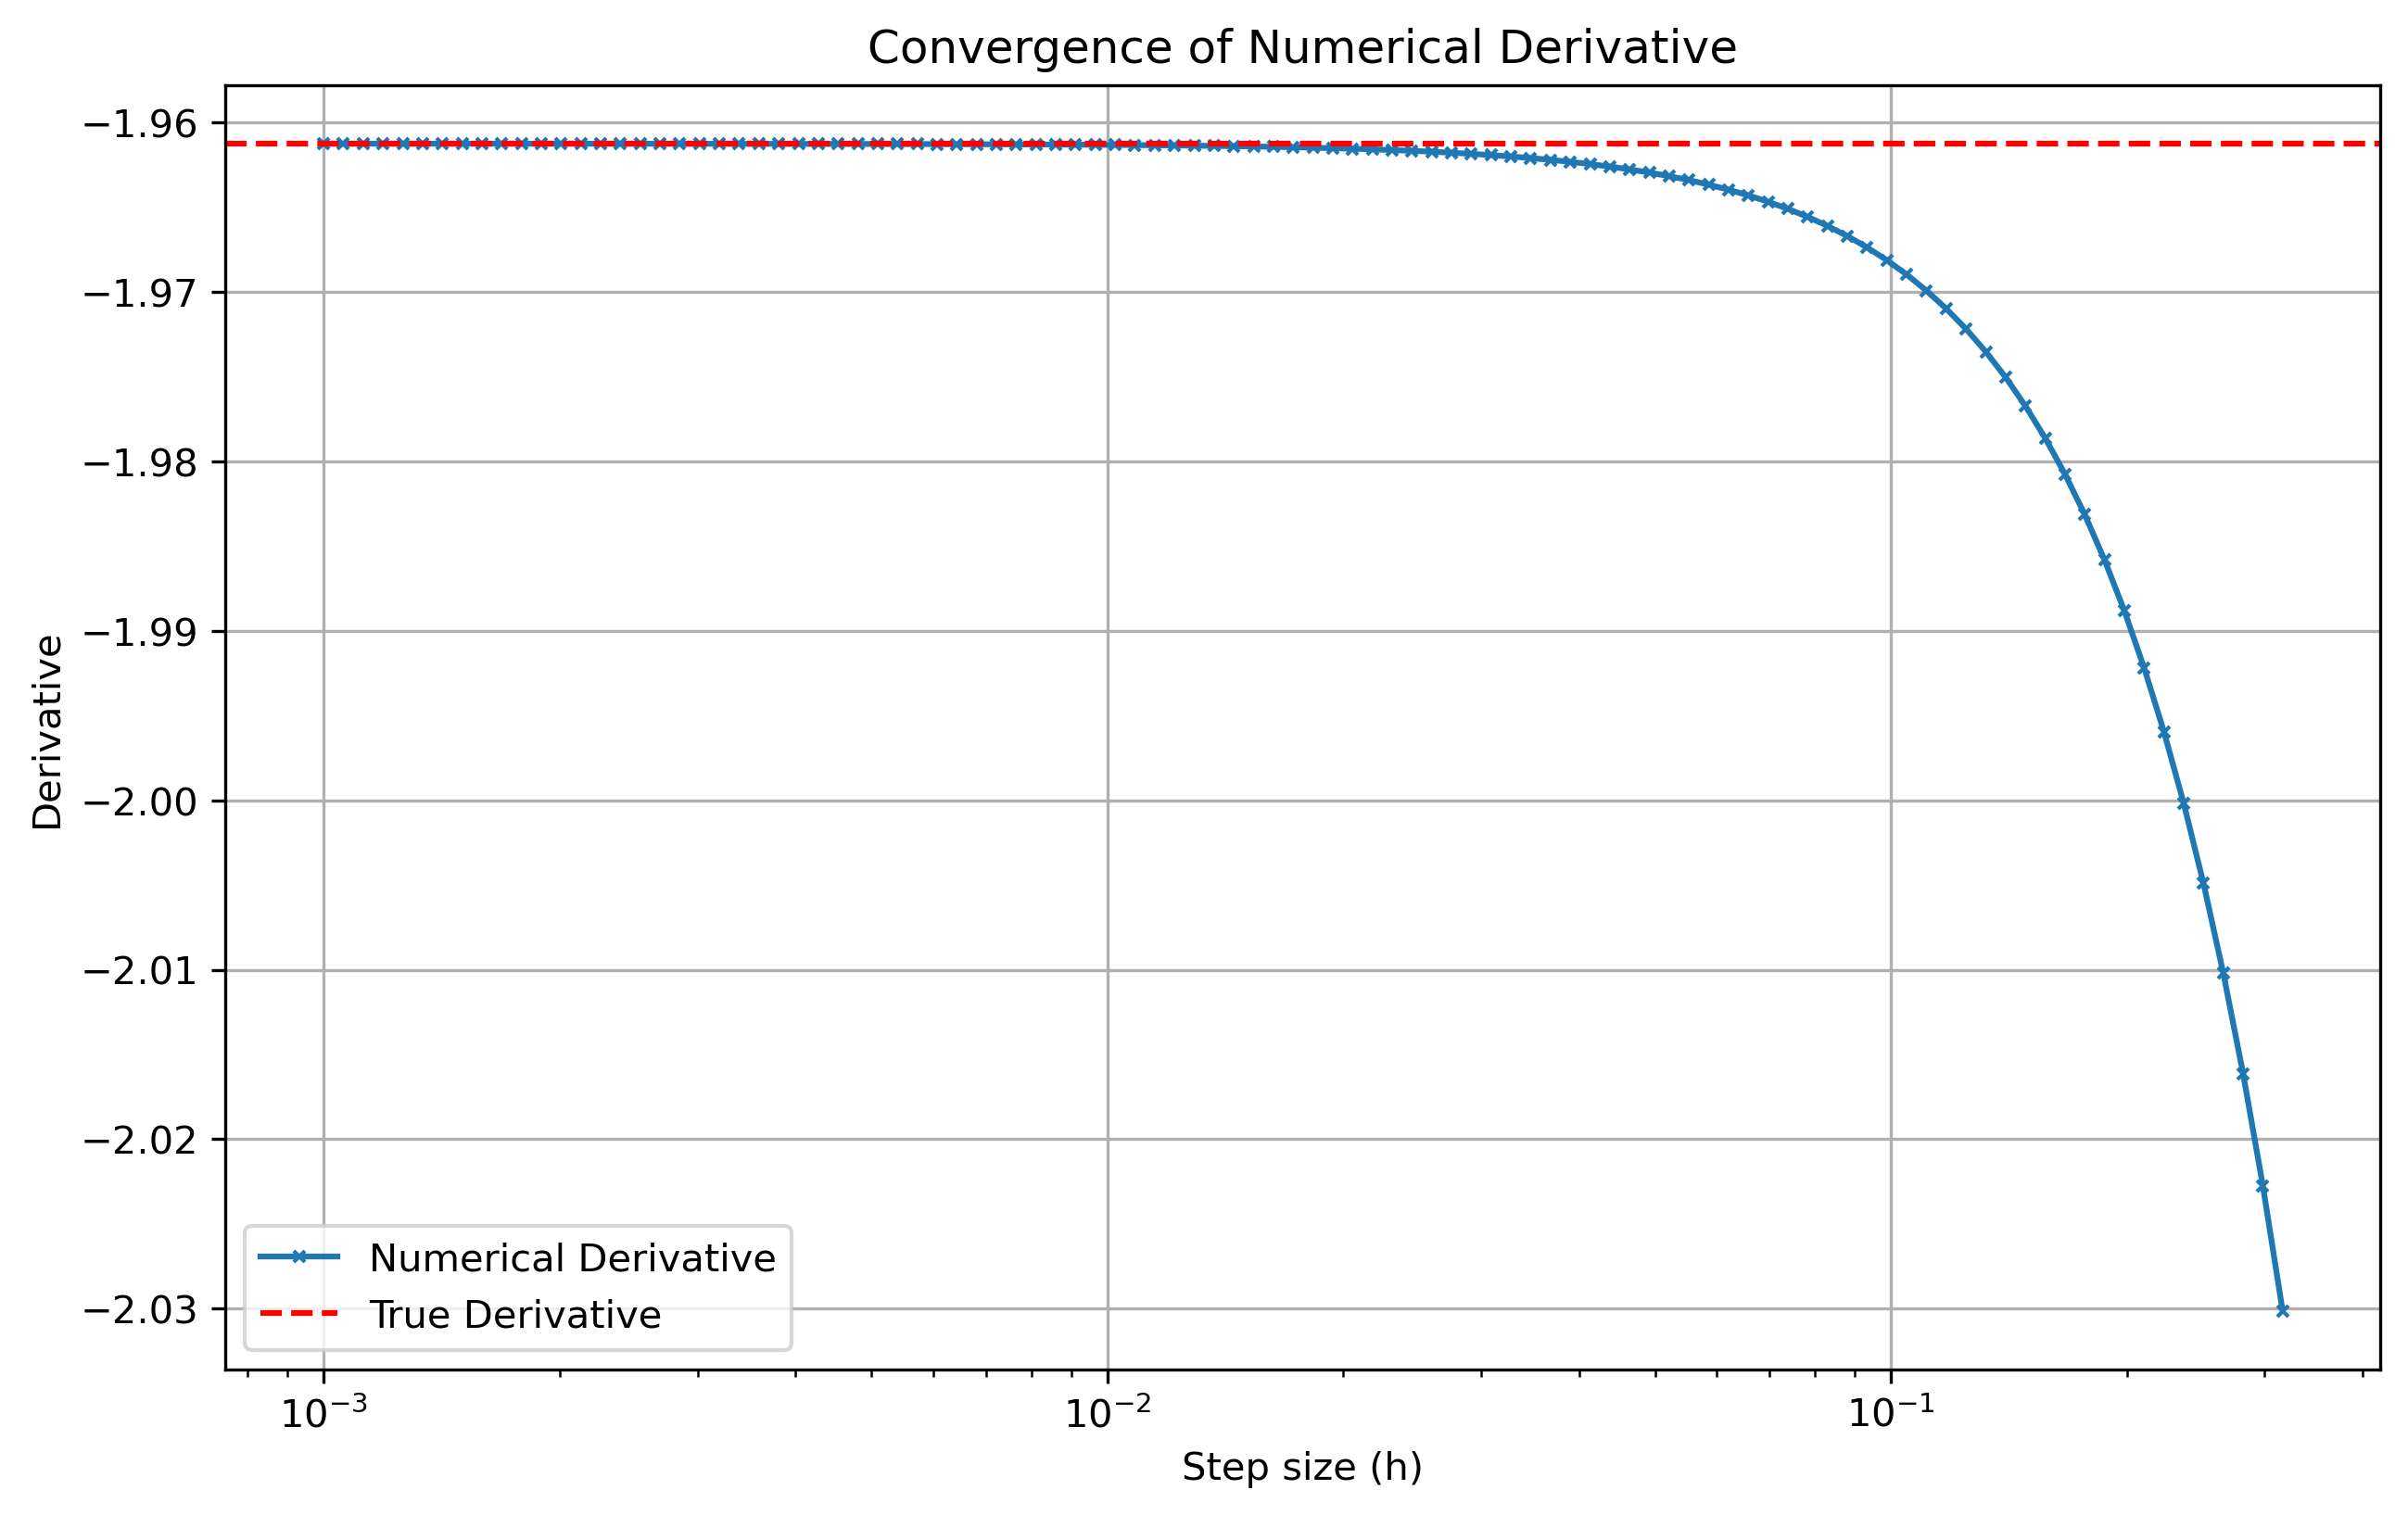
\includegraphics[width=0.8\textwidth]{convergence_derivative.png}
    \caption{Convergence of the numerical derivative for decreasing step sizes. The red dashed line indicates the true derivative obtained using dual numbers. The numerical derivative converges to the true value for small step sizes, but diverges due to round-off errors as \(h\) becomes excessively small.}
    \label{fig:convergence_derivative}
\end{figure}

\begin{itemize}
    \item \textbf{Accuracy:} For moderate values of \(h\), the numerical derivative closely matches the true value. However, as \(h\) increases further, round-off errors lead to divergence.
    \item \textbf{Dual Numbers:} The dual number method provides a stable and precise derivative, unaffected by the limitations of finite differences.
    \item \textbf{Efficiency:} Unlike numerical differentiation, dual numbers compute the derivative in a single step, making the method both computationally efficient and less error-prone.
\end{itemize}

\section{Tests and Validation}

The \texttt{tests/} directory contains unit tests designed to validate the functionality of the \texttt{dual\_autodiff} package. These tests ensure the correctness of mathematical operations, dual number functionality, and integration with various functions like trigonometric, logarithmic, and exponential operations.

\subsection{Structure of the \texttt{tests/} Directory}
The directory includes the following key test files:
\begin{itemize}
    \item \texttt{test\_dual.py}: Validates the core \texttt{Dual} class, including arithmetic operations and function implementations.
    \item \texttt{test\_functions.py}: Tests global mathematical functions like \texttt{sin}, \texttt{cos}, and \texttt{log}.
    \item \texttt{test\_base.py}: Ensures utility functions such as \texttt{is\_dual\_instance()} and \texttt{ensure\_dual()} work correctly.
\end{itemize}

\subsection{Outcome}
The tests validate that the \texttt{dual\_autodiff} package functions as expected under various scenarios. They also confirm that dual numbers provide accurate derivatives.

\section{Project Documentation with Sphinx}

The \texttt{docs/} directory contains all the files required to generate the HTML documentation for the \texttt{dual\_autodiff} package using Sphinx. After running \texttt{make html} in the terminal, Sphinx processes the source files and generates structured HTML documentation, which can be found in the \texttt{build/html/} directory.

\subsection{Structure of the \texttt{docs/} Directory}
\begin{itemize}
    \item \texttt{Makefile} and \texttt{make.bat}: Used to build the documentation. The \texttt{Makefile} is for Unix-based systems, while \texttt{make.bat} is for Windows.
    \item \texttt{source/}: Contains the source files for the documentation:
    \begin{itemize}
        \item \texttt{index.rst}: The main landing page of the documentation, linking to other sections.
        \item \texttt{dual\_autodiff.rst}: Detailed API reference for the package, generated using the \texttt{autodoc} extension.
        \item \texttt{modules.rst}: Lists all the modules included in the \texttt{dual\_autodiff} package.
        \item \texttt{tutorial.rst}: A guide for using the package, linking to the tutorial notebook.
        \item \texttt{dual\_autodiff.ipynb}: A Jupyter notebook providing hands-on examples of the package's features.
        \item \texttt{apple\_silicon\_x86\_setup.rst}: A section explaining how to set up the development environment on Apple Silicon devices.
        \item \texttt{conf.py}: The Sphinx configuration file, which defines project settings, extensions, and theme configurations.
    \end{itemize}
    \item \texttt{build/}: Stores the generated documentation:
    \begin{itemize}
        \item \texttt{build/doctrees/}: Contains intermediate files generated during the build process.
        \item \texttt{build/html/}: The final HTML output, including static assets, search functionality, and individual pages:
        \begin{itemize}
            \item \texttt{index.html}: The main landing page.
            \item \texttt{dual\_autodiff.html}: Detailed API reference.
            \item \texttt{tutorial.html}: The tutorial section with examples.
            \item \texttt{apple\_silicon\_x86\_setup.html}: Instructions for configuring the development environment.
            \item \texttt{\_static/}: Contains CSS, JavaScript, and image assets for styling and functionality.
        \end{itemize}
    \end{itemize}
\end{itemize}

\subsection{Generated Output}
The generated HTML documentation features:
\begin{itemize}
    \item \textbf{Landing Page:} An overview of the project with links to tutorials and references.
    \item \textbf{API Reference:} Detailed documentation for all modules, classes, and functions in the package.
    \item \textbf{Tutorial:} A step-by-step guide, showcasing practical examples of using the package.
    \item \textbf{Environment Setup Guide:} Instructions for configuring the development environment on Apple Silicon devices.
\end{itemize}

The Sphinx-generated documentation ensures clarity and accessibility, providing users with a detailed understanding of the \texttt{dual\_autodiff} package. It combines automatically generated API references with user-friendly tutorials, making it an essential resource for both developers and users.

\section{Cythonizing the Package}

\subsection{Overview of Configuration Files}
To Cythonize the \texttt{dual\_autodiff} package, several configuration files were created and customized to streamline the process. These include:

\subsubsection{\texttt{setup.py}}
The \texttt{setup.py} file defines the build process for the Cython extensions. It:
\begin{itemize}
    \item Reads metadata such as the package name, version, and description from the \texttt{README.md}.
    \item Specifies Cython modules (e.g., \texttt{dual.pyx}, \texttt{functions.pyx}) to be compiled.
    \item Uses \texttt{setuptools} and \texttt{cythonize} to compile Python files into C extensions.
    \item Excludes unnecessary source files (e.g., \texttt{.pyx}, \texttt{.py}) from the final package to ensure only compiled files are distributed.
\end{itemize}

\subsubsection{\texttt{pyproject.toml}}
The \texttt{pyproject.toml} file manages project metadata and build system requirements. It:
\begin{itemize}
    \item Specifies the package name, version, description, and homepage URL.
    \item Declares \texttt{setuptools}, \texttt{Cython}, and \texttt{wheel} as build dependencies.
    \item Ensures compatibility with Python 3.6 and higher.
\end{itemize}

\subsubsection{\texttt{MANIFEST.in}}
The \texttt{MANIFEST.in} file controls which files are included or excluded in the package distribution. It:
\begin{itemize}
    \item Includes essential files such as \texttt{README.md}, \texttt{setup.py}, and \texttt{pyproject.toml}.
    \item Recursively includes compiled shared object files (\texttt{.so}).
    \item Excludes intermediate files generated during compilation (e.g., \texttt{.c}, \texttt{.cpp}, \texttt{.h}).
\end{itemize}

\subsection{Cythonization Steps}
\begin{enumerate}
    \item \textbf{Organizing the Code:}
    The source files from the \texttt{dual\_autodiff} directory were copied into a new directory named \texttt{dual\_autodiff\_x} to create a separate namespace for the Cythonized implementation.

    \item \textbf{Renaming Files:}
    The Python files (\texttt{.py}) for core functionality, including \texttt{dual.py}, \texttt{functions.py}, and \texttt{base.py}, were renamed to \texttt{.pyx}. This step is essential because Cython requires source files to have the \texttt{.pyx} extension for compilation.

    \item \textbf{Setting Up Configuration Files:}
    The following configuration files were created and customized:
    \begin{itemize}
        \item \texttt{setup.py}: Defined the extensions to be compiled and specified Cython directives (e.g., Python 3 language level).
        \item \texttt{pyproject.toml}: Declared build dependencies such as \texttt{setuptools}, \texttt{wheel}, and \texttt{Cython}.
        \item \texttt{MANIFEST.in}: Included necessary files (e.g., compiled shared objects) and excluded temporary source files.
    \end{itemize}

    \item \textbf{Compiling and Installing the Modules:}
The Cython source files (\texttt{.pyx}) were compiled into shared object files (\texttt{.so}) and the package was installed in editable mode for testing and further development. This was done using the following commands:
\begin{verbatim}
python setup.py build_ext --inplace
pip install -e .
\end{verbatim}
\end{enumerate}

\section{Performance Comparison: Pure Python vs. Cythonized Version}

To assess the performance improvement achieved through Cythonization, a comparative analysis of the pure Python and Cythonized versions of the \texttt{dual\_autodiff} package was conducted. The execution time for both implementations was measured as a function of the array length (number of dual numbers) across varying ranges of dual numbers. The key observations are summarized below.

\subsection{Experimental Setup}
Execution times were measured using a test function on arrays of dual numbers with lengths from 100 to 14,000, and real parts drawn from three ranges: 
(0,10), (10,100), and (100,1000). Each experiment was repeated 100 times for consistency. Linear regression was applied to compute gradients, quantifying the computational efficiency of both Python and Cythonized implementations.
\begin{figure}[h!]
    \centering
    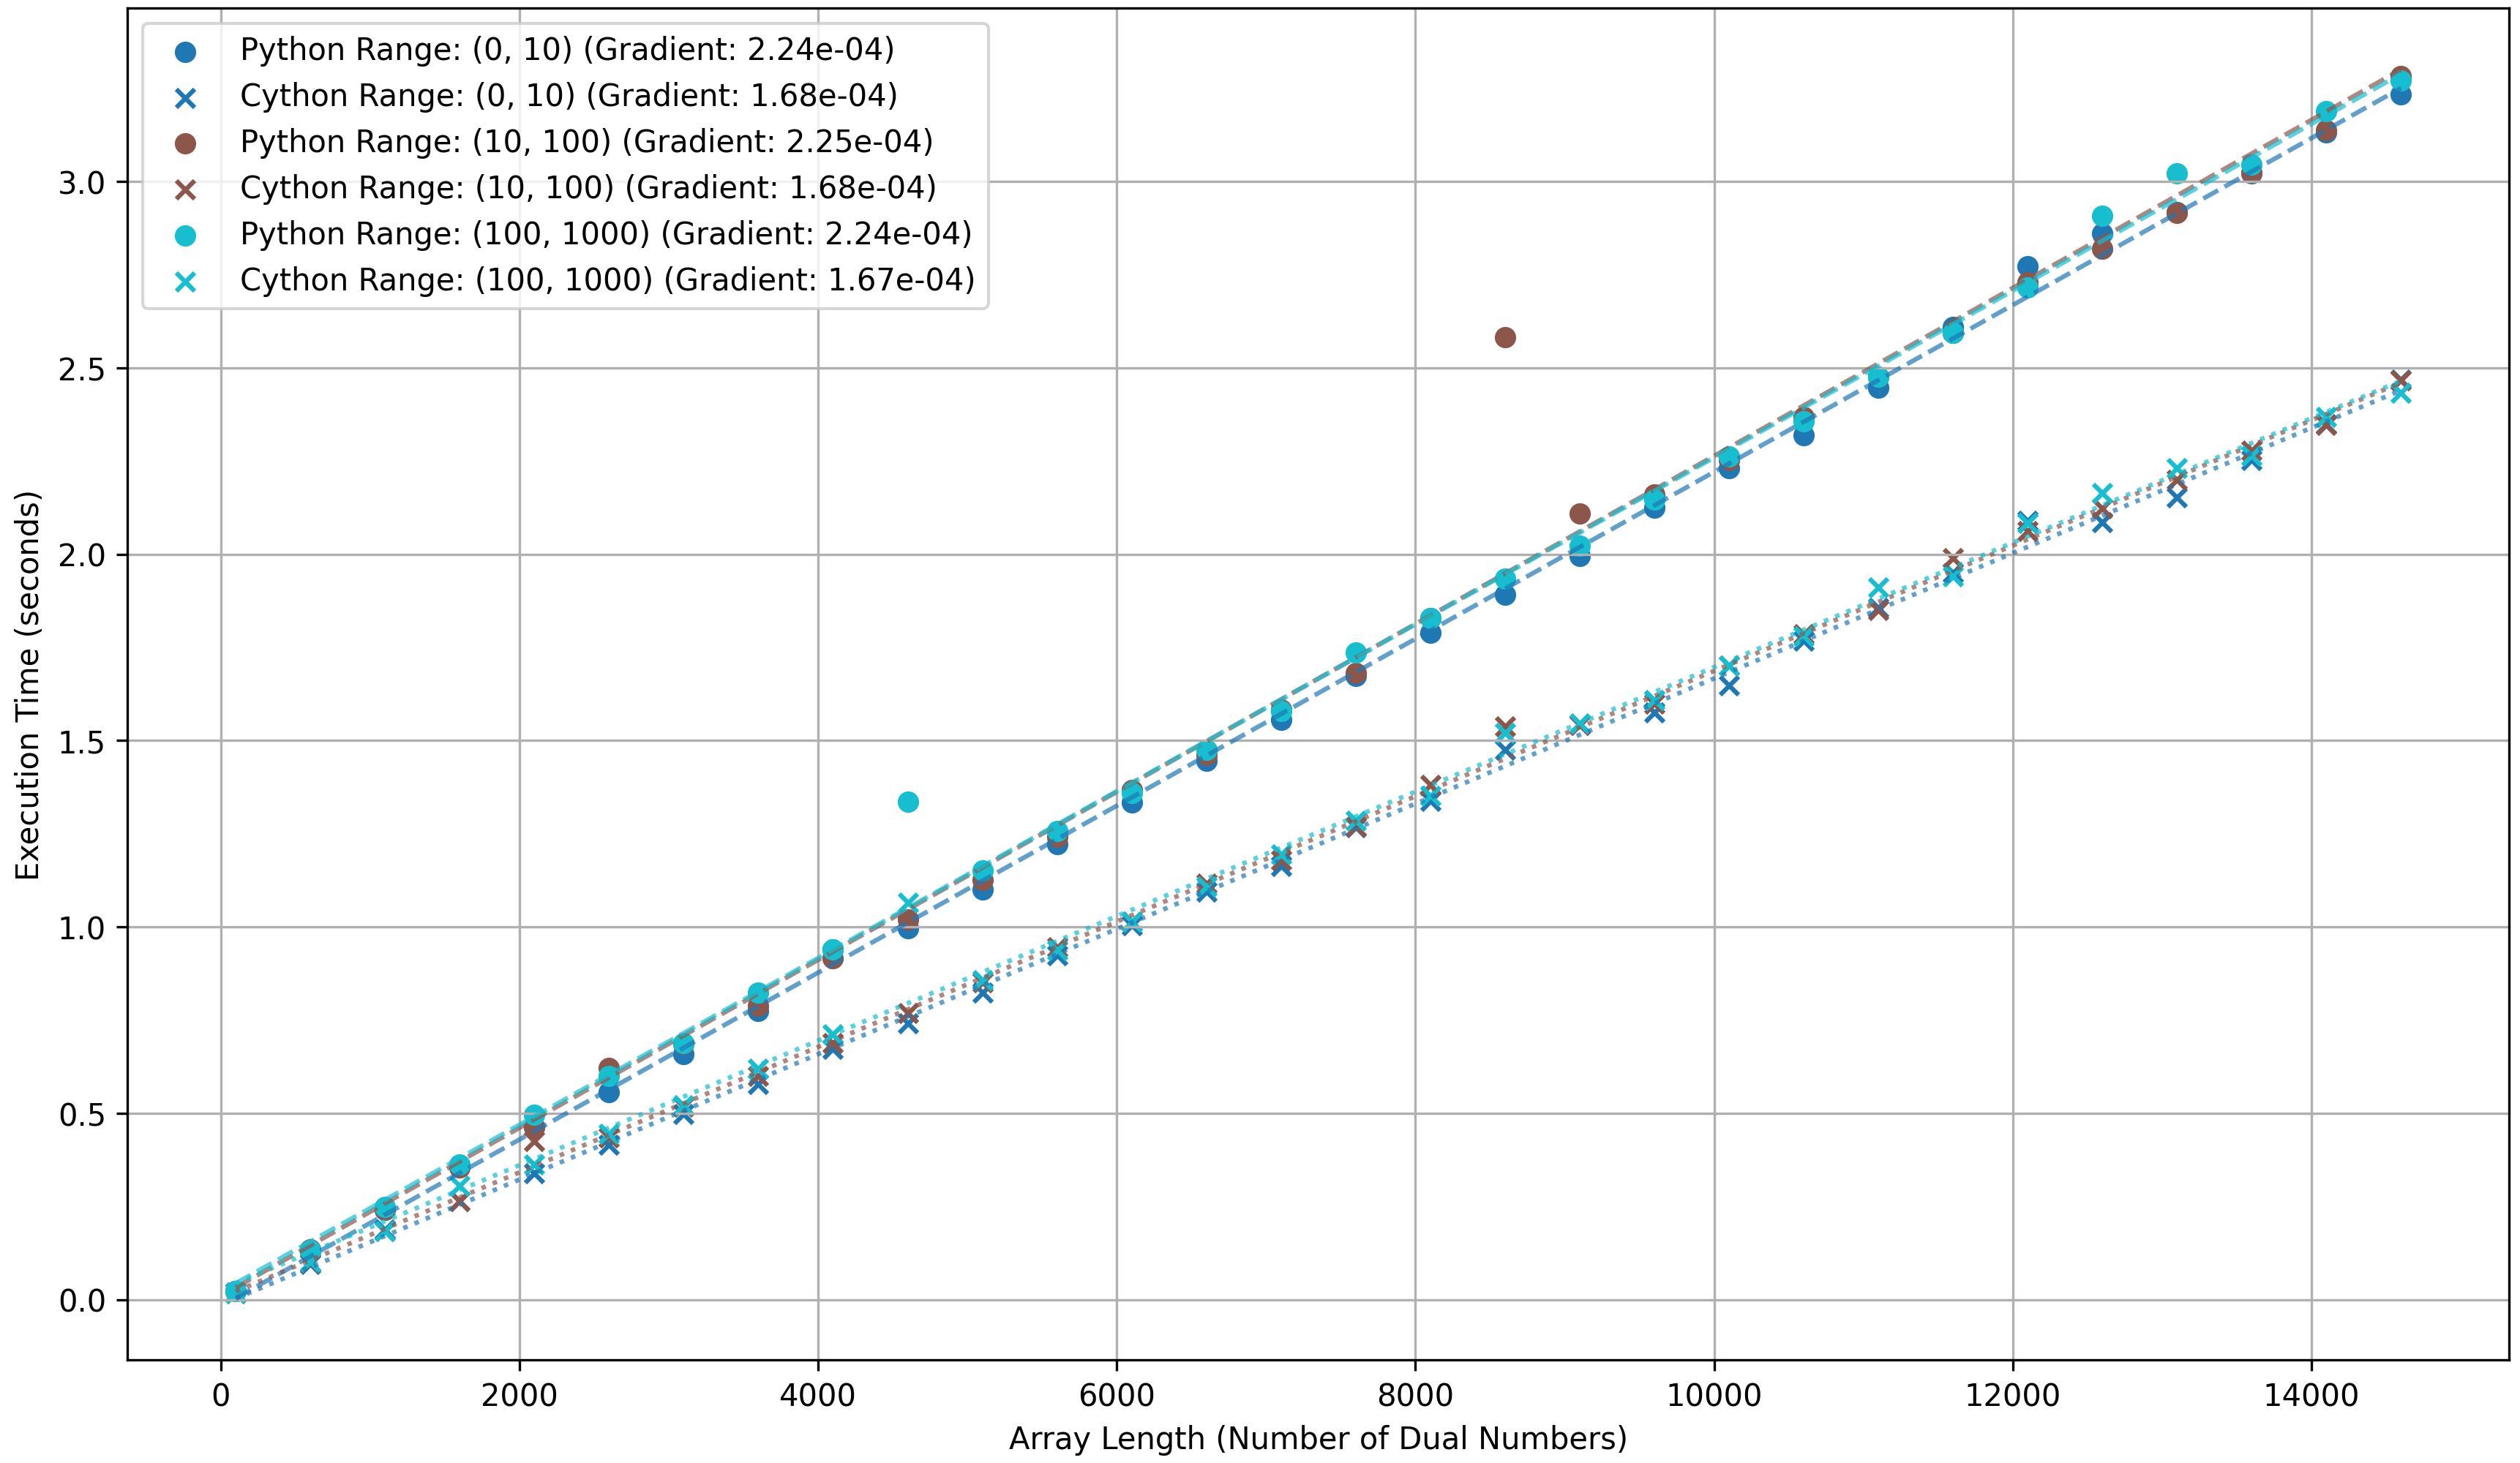
\includegraphics[width=0.8\textwidth]{performance_comparison.png}
    \caption{Performance comparison between the pure Python and Cythonized versions of \texttt{dual\_autodiff}. The plot shows execution times as a function of array length for three different ranges of dual numbers. The gradients indicate the rate of increase in execution time with array length.}
    \label{fig:performance_comparison}
\end{figure}

\subsection{Results and Observations}
Figure~\ref{fig:performance_comparison} shows the execution times of the pure Python and Cythonized versions for the three ranges of dual numbers. The following observations were made:
\begin{itemize}
    \item The Cythonized version consistently outperformed the pure Python version across all ranges, demonstrating lower execution times for equivalent array lengths.
    \item The gradients of the execution times (indicated in the legend) were smaller for the Cythonized version, indicating better scalability with increasing array lengths.
    \item The performance difference was more pronounced for larger arrays, highlighting the advantage of Cythonized code in computationally intensive scenarios.
\end{itemize}

\subsection{Analysis of Gradients}
The gradients of the execution time with respect to the array length, as indicated in the legend of Figure~\ref{fig:performance_comparison}, provide a quantitative measure of the computational efficiency of the Python and Cythonized versions. These gradients represent the rate at which execution time increases with the number of dual numbers in the array. The following insights can be drawn from the gradients:

\subsection{Analysis of Gradients}
The gradients in Figure~\ref{fig:performance_comparison} provide a quantitative measure of how execution time scales with the array length:

\begin{itemize}
    \item \textbf{Python Implementation:} The gradients are consistently higher, around \(2.20 \times 10^{-4}\), across all ranges of dual numbers. This indicates that the execution time for the Python implementation increases more rapidly with the number of dual numbers. The similarity of gradients across ranges suggests that the range of real parts has minimal impact, and the computational overhead primarily depends on array length.
    
    \item \textbf{Cythonized Implementation:} The gradients are significantly lower, approximately \(1.63 \times 10^{-4}\), for all ranges. This slower rate of increase in execution time highlights the efficiency of the Cythonized implementation. A lower gradient indicates that the Cythonized version scales better with increasing array lengths, making it more suitable for handling larger datasets.
\end{itemize}

\textbf{Scalability and Impact of Lower Gradients:} \\
The lower gradient for the Cythonized implementation demonstrates its superior scalability. As the array length grows, the execution time for the Cythonized version increases at a much slower rate compared to the Python implementation. This efficiency arises from the reduced overhead in Cython, where the code is compiled into C, minimizing dynamic type-checking and interpretation, which are inherent to Python. Consequently, the Cythonized version is better equipped to handle larger and more computationally intensive tasks efficiently.

\section{Building Wheels for Linux}

To create specific wheels for the \texttt{dual\_autodiff\_x} package targeting \texttt{cp310-manylinux\_x86\_64} and \texttt{cp311-manylinux\_x86\_64}, the process was carried out manually on the University of Cambridge's CSD3 cluster due to compatibility issues on macOS M4.

\subsection{Steps for Building the Wheels}
\begin{enumerate}
    \item \textbf{Building the Python 3.10 Wheel:}
    \begin{itemize}
        \item Python 3.10 was built from source and installed in \texttt{\$HOME/python310}:
        \begin{verbatim}
        ./configure --prefix=$HOME/python310 --enable-optimizations
        make -j$(nproc) && make install
        \end{verbatim}
        \item The wheel was created and saved in the \texttt{wheelhouse} directory:
        \begin{verbatim}
/home/rsr45/python310/bin/python3.10 setup.py bdist_wheel --dist-dir wheelhouse
        \end{verbatim}
    \end{itemize}

    \item \textbf{Building the Python 3.11 Wheel:}
    \begin{itemize}
        \item Verified Python 3.11 was installed on CSD3 and prepared the environment:
        \begin{verbatim}
        python3.11 -m pip install --user --upgrade pip setuptools wheel cython
        \end{verbatim}
        \item The wheel was created and saved in the \texttt{wheelhouse} directory:
        \begin{verbatim}
        python3.11 setup.py bdist_wheel --dist-dir wheelhouse
        \end{verbatim}
    \end{itemize}
\end{enumerate}

\subsection{Contents of the Wheel}
The built wheels for Python 3.10 and 3.11 were inspected to ensure they contained the necessary compiled binaries and metadata for distribution. The key contents included:

\begin{itemize}
    \item \textbf{Compiled Binaries:} The \texttt{dual\_autodiff} directory contained shared object files (\texttt{*.so}) for the core modules (\texttt{base}, \texttt{dual}, and \texttt{functions}), ensuring optimized performance without exposing the source code.
    \item \textbf{Metadata:} The \texttt{dist-info} directory included essential metadata files such as:
    \begin{itemize}
        \item \texttt{METADATA}: Package details like name, version, and dependencies.
        \item \texttt{WHEEL}: Compatibility and wheel-specific metadata.
        \item \texttt{RECORD}: File integrity and hash information.
    \end{itemize}
\end{itemize}






\printbibliography


\end{document}
